To evaluate the impact of our scheduler, we compare the two approaches from Section \ref{sec:scalability} to our interleaving scheduler which aims to satisfy the \enquote{Optimum} solution. Additionally, we use the sequential scheduling algorithm as baseline while synchronous scheduling represents the worst case by forcing maximum interference. All scenarios are considered in terms of total autotuning completion time, time for the individual stages and the resulting inference performance.

Our evaluation environment consists of two identical machines with the following specifications:
\begin{itemize}
	\item 2x Intel Xeon E5-2650 v3, 10 cores, \SI{2.30}{\giga\hertz}
	\begin{itemize}
		\item Hyper-threading enabled
		\item AVX2 instruction set
	\end{itemize}
	\item \SI{128}{\giga\byte} main memory
	\item 4x Tesla K80 \glspl{gpu}, 4992 CUDA cores, \SI{24}{\giga\byte} memory
	\item Ubuntu 16.04.6 with Linux Kernel 4.4.0
	\item Python 3.6.8
\end{itemize}

Clients always run on the first machine, while profiling servers (TVM RPC servers) always run on the second machine whose \glspl{gpu} are used as target devices. Scheduler and tracker run on the first machine to decrease network latency. They do not interfere with autotuning since they are not computationally intensive.

The number of clients and profiling servers changes for every experiment, as shown in Table \ref{tab:tvm-evaluation-setups}. On \enquote{dedicated} servers, there is only one client. Two clients run on \enquote{shared} servers. Each profiling server of one client is assigned to a different GPU. Without interleaving, each client has its own set of four profiling servers, which might result in two servers if different clients being assigned to the same GPU. However, with interleaving, they can share the servers since they will never profile at the same time, eliminating competition.
\begin{table}
	\newcommand\heading[1]{\textcolor{white}{\textbf{#1}}}
	\renewcommand{\arraystretch}{1.2}
	\sffamily
	\centering
	\begin{tabularx}{\textwidth}{l l l l X}
	\rowcolor{black} \heading{Setup} & \heading{Server~~~~~} & \heading{Scheduler~~~~~~~~~~~~~} & \heading{Bundling~~~} & \heading{Profiling servers} \vspace{2pt} \\
	\textbf{A} & Dedicated & sequential & No & 4 \\
	\textbf{B} & Shared & sequential & No & 8 \\
	\textbf{C} & Shared & synchronous & No & 8 \\
	\textbf{D} & Shared & interleaved-greedy & No & 4 \\
	\textbf{E} & Shared & interleaved-fair & No & 4 \\
	\textbf{F} & Shared & interleaved-greedy & Yes & 4 \\
	\textbf{G} & Shared & interleaved-fair & Yes & 4 \\
	\end{tabularx}
	\caption{Evaluation setups}
	\label{tab:tvm-evaluation-setups}
\end{table}

All setups are controlled by the scheduler so each experiment is affected by the---albeit minimal---overhead of scheduling and \gls{rpc}. Two separate schedulers, one for each client, are used in B to achieve natural interference. \enquote{Bundling} indicates if stages of one resource are bundled into a single stage using the \pythoninline/BundlingJobManager/, or if each stage is individually scheduled.

Our test model is a ResNet-18, which consists of 12 convolution layers and one fully-connected layers, resulting in a job of 13 tasks. We autotune with 2000 trials per task and a profiling timeout of \SI{5}{\second}. Transfer learning from the global autotuning database is disabled so each experiment starts from the same, untrained cost model for a fair comparison. However, transfer learning is enabled between tasks. For time reasons, each experiment is only conducted once so the sample size is small.

A complete chart of all results can be found in Appendix \ref{sec:results}.

\section{Results}
First, we examine the impact of interference that was qualitatively described in Section \ref{sec:scalability}. We compare A, the optimum in terms of autotuning time and inference performance, with B and C (Figure \ref{fig:chart-interference-impact}). B lets jobs naturally interfere, while C forces maximum interference as worst case scenario. Interference is particularly noticeable for model updates since they are rather computationally intensive, which is why we show model update time in every figure.\\
The baseline completion time from A is \SI{14.5}{\hour}, \SI{6.1}{\hour} (42\%) of which are spent updating the model. Natural interference results in an increase in autotuning time by \SI{4.1}{\hour} (+28\%) while forced interference takes even \SI{5.0}{\hour} (+34\%) longer\footnote{For C, the time spent waiting for the other job to finish a stage introduced by the synchronous scheduling algorithm to force interference was subtracted from the total completion time since it would not occur naturally.}. This significant increase can be attributed to slower model updates, which witness a strong decline in performance. Compared with the baseline, the total time spent updating the model increases by \SI{3.8}{\hour} (+62\%) for B and by \SI{5.2}{\hour} (+85\%) for C. Build time only increases marginally, with profiling being slightly faster, possibly due to more timeouts. The baseline inference time is \SI{48.6}{\milli\second}. B is \SI{1.5}{\milli\second} slower, C is \SI{0.5}{\milli\second} slower. 

\begin{figure}[t]
	\begin{minipage}[b]{.6\textwidth}
		\centering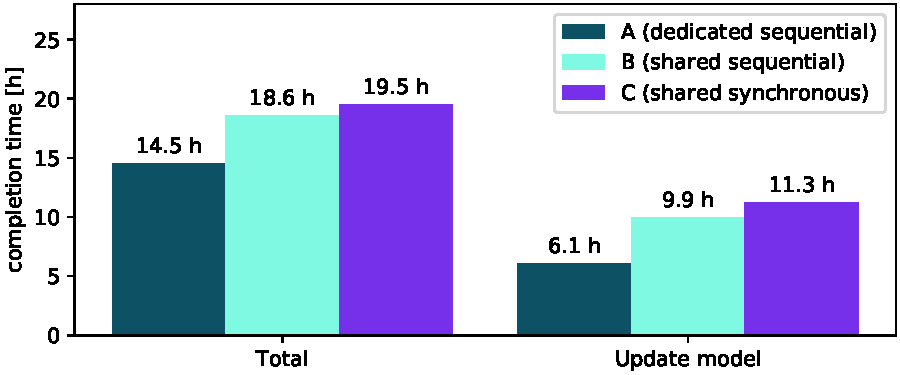
\includegraphics[width=\textwidth]{chart_interference_impact_completion}
		\subcaption{Completion time}\label{fig:chart-interference-impact-completion}
	\end{minipage}%
	\hfill
	\begin{minipage}[b]{.35\textwidth}
		\centering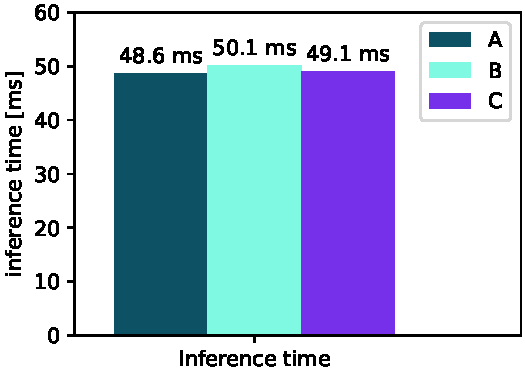
\includegraphics[width=\textwidth]{chart_interference_impact_inference}
		\subcaption{Inference performance}\label{fig:chart-interference-impact-inference}
	\end{minipage}
	\caption{Impact of interference}
	\label{fig:chart-interference-impact}
\end{figure}

We examine experiments D and E to evaluate the greedy and fair scheduler algorithm design, comparing them with A as baseline (Figure \ref{fig:chart-interleaving}). Using greedy interleaving, autotuning completes in \SI{20.4}{\hour}, \SI{5.9}{\hour} slower than A. While model update time stays about the same, \SI{5.5}{\hour} (27\%) of the total time is now spent waiting\footnote{Only stage execution times can be measured. Wait time and non-stage times (transfer learning, file operations) need to be derived. Non-stage times are about \SI{0.49}{\hour}, derived from A. Wait time for interleaving is calculated as follows: $t_{wait} = t_{total} - \sum_{i}t_{stage,i} - \SI{0.49}{\hour}$} for resources to become free to prevent interference. Fair interleaving is impacted even more by waiting, with total autotuning time increasing to \SI{24.1}{\hour}, \SI{9.6}{\hour} (+62\%) slower than A. Model update time remains about the same again, but wait time accumulates to \SI{8.9}{\hour} (37\% of total autotuning). Building and profiling time do not change for both. While the total completion time deteriorates, inference performance matches the baseline of \SI{48.6}{\milli\second} for both D and E.

\begin{figure}[t]
	\begin{minipage}[b]{.6\textwidth}
		\centering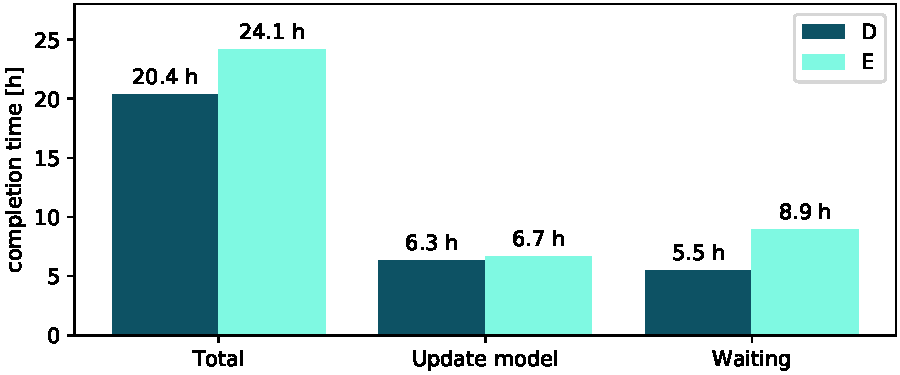
\includegraphics[width=\textwidth]{chart_interleaving_completion}
		\subcaption{Completion time}\label{fig:chart-interleaving-completion}
	\end{minipage}%
	\hfill
	\begin{minipage}[b]{.35\textwidth}
		\centering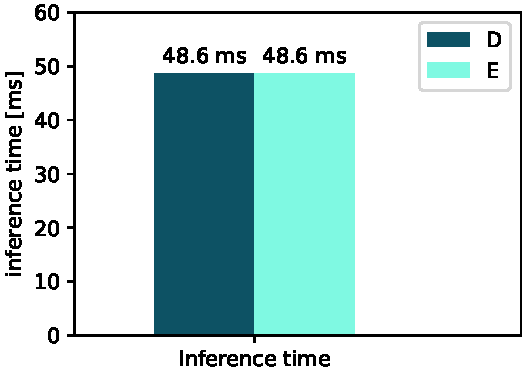
\includegraphics[width=\textwidth]{chart_interleaving_inference}
		\subcaption{Inference performance}\label{fig:chart-interleaving-inference}
	\end{minipage}
	\caption[Results of greedy versus fair interleaving]{Greedy versus fair interleaving}
	\label{fig:chart-interleaving}
\end{figure}

Finally, we examine the effect of employing stage bundling as opposed to individually scheduling them (Figure \ref{fig:chart-bundling}). The greedy algorithm is used in F, the fair algorithm is used in G. With bundling, greedy interleaving performs about the same as without bundling. On the other hand, fair interleaving completes \SI{2.4}{\hour} (-10\%) earlier than the individually scheduled version due to a total wait time that is \SI{2.7}{\hour} (-30\%) shorter. As before, model update time remains relatively similar. Inference time in F is \SI{0.4}{\milli\second} faster than in D, while G's is slower by \SI{1.3}{\milli\second}.

\begin{figure}[t]
	\begin{minipage}[b]{.6\textwidth}
		\centering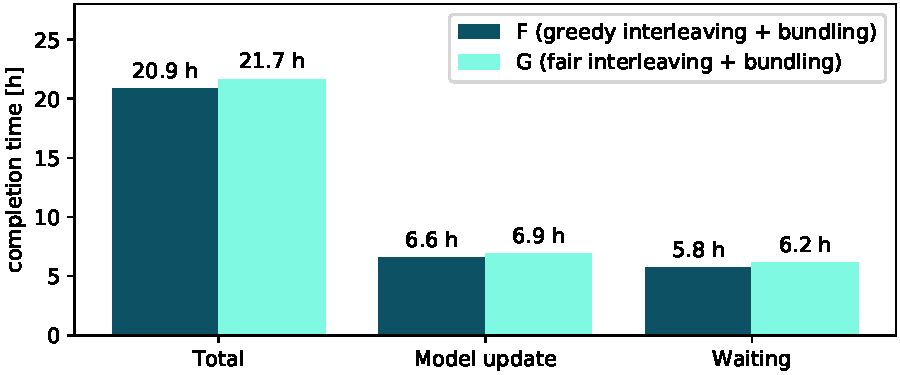
\includegraphics[width=\textwidth]{chart_bundling_completion}
		\subcaption{Completion time}\label{fig:chart-bundling-completion}
	\end{minipage}%
	\hfill
	\begin{minipage}[b]{.35\textwidth}
		\centering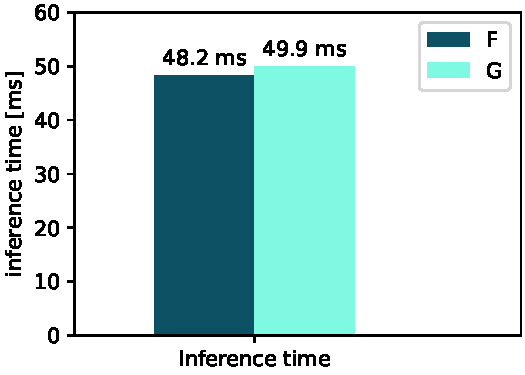
\includegraphics[width=\textwidth]{chart_bundling_inference}
		\subcaption{Inference performance}\label{fig:chart-bundling-inference}
	\end{minipage}
	\caption[Results of greedy versus fair interleaving with bundling]{Greedy versus fair interleaving with bundling}
	\label{fig:chart-bundling}
\end{figure}

\section{Discussion}
The objective of large-scale autotuning is to achieve the autotuning time and inference performance of running only a single job on each server, but with shared resources to keep the amount of required hardware at a minimum. Single-job autotuning is represented by Setup A, which is why we use it as baseline for comparisons with the other experiments. Because our evaluation is limited to a single machine type and model, more experiments are required for a general analysis.

In B and C we show the detrimental effects of interference on performance which motivated the creation of a scheduler. If it were not for this, resources could be shared and jobs could be run in parallel without control by a central entity. B and C behave relatively similar because even without explicit scheduling, both jobs run approximately synchronous since they autotune the same model. In real-world scenarios with diverse workloads, there might be a more drastic difference between B and C. The fact that C has faster inference than B is presumably caused by the probabilistic nature of configuration selection. The difference in inference performance of both to the baseline is relatively small due to the large number of trials which even out the impact of interference. However, even slightly worse inference speed has a large impact with an increasing number of inferences.

Note how interference is avoided with the scheduler in D--G, which manifests in stage times (particularly model updating) that are comparable to single-job autotuning as well as in a good inference performance. However, a significant amount of wait time is introduced which drives up total completion time. Greedy interleaving without bundling shows the shortest wait time in our experiments. Bundling does not show a big effect when comparing D and F because greedy interleaving naturally behaves like bundling. However, fair interleaving benefits much from bundling in our experiments, remedying the vast wait time. Inference performance is not optimal in G, more experiments might yield a better result.

Greedy interleaving works well in our experiments because both jobs are identical and the portion of time spent on the client machine versus time spent on the target device is roughly similar. As a result, wait time is reduced because, after an initial wait period, both jobs alternate nearly perfectly but mutually opposing between client and target. Despite these results, we believe that fair interleaving is the superior algorithm for scheduling heterogeneous jobs with varying complexity on a large scale, as would be the case with \gls{aaas}. Greedy interleaving would allow jobs to monopolize resources for an extended period of time, while fair interleaving allows for a finer control, especially if more resources are available. Bundling in conjunction with the fair algorithm is still an option to interleave homogeneous jobs on few resources, which would show the same effect as the greedy algorithm in our experiment.

Our scheduler is very rudimentary at this point, leaving much room for improvement. While the concept of interleaving seems promising, a more intelligent approach than fair round-robin could be employed to fill idle time optimally while keeping average wait time low. For example, a predictive scheduler could use knowledge from previous tasks to make a more educated decision that will maximize resource utilization. This would augment the notion of load-awareness with knowledge about the estimated stage execution time. Such a scheduler could then leverage the exact or heuristic interleaving algorithm from \cite{Ma.2005}. However, a more sophisticated algorithm might require finer control over the stages, which cannot be provided by the client's current resource/stage interface. Trading off a complex client but simple scheduler for a thin, stateless client and autotuning-aware scheduler by shifting responsibilities might become a necessity.

Furthermore, the scheduler needs to be enhanced with support for multiple resources of the same type. At this point, all target devices are regarded as a single, atomic resource. More granularity is essential for production-grade implementations in an \gls{aaas} platform. This would go hand in hand with eliminating the tracker and letting the scheduler assign target devices to clients. A trivial refinement is replacing the busy waiting for a stage to be done in the scheduler algorithm, resulting in an excess of redundant \gls{rpc} calls, by a push-based approach, where the client notifies the scheduler once a stage has completed.

We used our scheduler only for autotuning with TVM. However, other autotuning frameworks like \gls{tc} that have the same scaling issues might also profit from our solution. The \gls{aaas} platform might even provide support for a variety of autotuning frameworks.